\chapter{Конструкторский раздел}\label{design}

\section{Требования к разрабатываемому методу}

Разрабатываемый метод должен обеспечивать согласованную обработку логически значимых игровых событий в условиях асинхронного сетевого обмена. 
Под логически значимым событием понимается событие, приводящее к изменению состояния игрока, общего игрового объекта или состояния взаимодействия между двумя игроками.

К методу синхронизации предъявляются следующие требования:
\begin{itemize}
	\item метод должен описывать взаимодействие двух игроков как обработку событий, вызывающих допустимые переходы конечного автомата синхронизируемого объекта;
	\item обработка критичных событий должна выполняться через авторитетный сервер, проверяющий порядок сообщений и допустимость применения события;
	\item каждое событие, изменяющее состояние системы, должно иметь уникальный идентификатор;
	\item каждое событие должно иметь номер последовательности в потоке событий игрока-отправителя;
	\item повторное получение одного и того же события не должно приводить к повторному изменению состояния;
	\item потеря события или подтверждения должна обнаруживаться на прикладном уровне;
	\item неподтвержденные события должны повторно отправляться до получения подтверждения;
	\item события, недопустимые для целевого конечного автомата, должны отклоняться;
	\item метод должен учитывать возможность задержки, потери, дублирования и нарушения порядка доставки UDP-пакетов.
\end{itemize}

Ограничением метода является рассмотрение взаимодействия двух игроков. Такое ограничение позволяет явно описать события и состояния игровых объектов, 
не вводя дополнительные механизмы масштабирования.

\section{Функциональная модель метода}

Разрабатываемый метод использует клиент-серверную схему обмена. Клиент формирует событие по локальному действию игрока и отправляет его серверу по UDP. 
Сервер выступает авторитетной стороной. Он проверяет событие, применяет его к целевому конечному автомату, отправляет подтверждение игроку-отправителю и рассылает подтвержденное событие клиентам.

Метод синхронизации включает следующие основные этапы:
\begin{enumerate}
	\item формирование локального игрового события на стороне клиента;
	\item присвоение событию идентификатора и номера последовательности;
	\item отправка события серверу;
	\item сохранение события в журнале неподтвержденных событий клиента;
	\item получение события сервером;
	\item проверка идентификатора события и фильтрация дубликатов;
	\item проверка номера последовательности события;
	\item поиск целевого объекта по идентификатору;
	\item применение события к конечному автомату целевого объекта;
	\item отправка подтверждения клиенту-отправителю;
	\item рассылка подтвержденного события клиентам;
	\item удаление подтвержденного события из журнала неподтвержденных событий клиента.
\end{enumerate}


Декомпозиция функции обеспечения согласованности состояний приведена на рисунке~\ref{img:design-idef0}. 
Она отражает последовательность обработки события от формирования на стороне клиента до подтверждения обработки и распространения результата.

\begin{figure}[H]
	\centering
	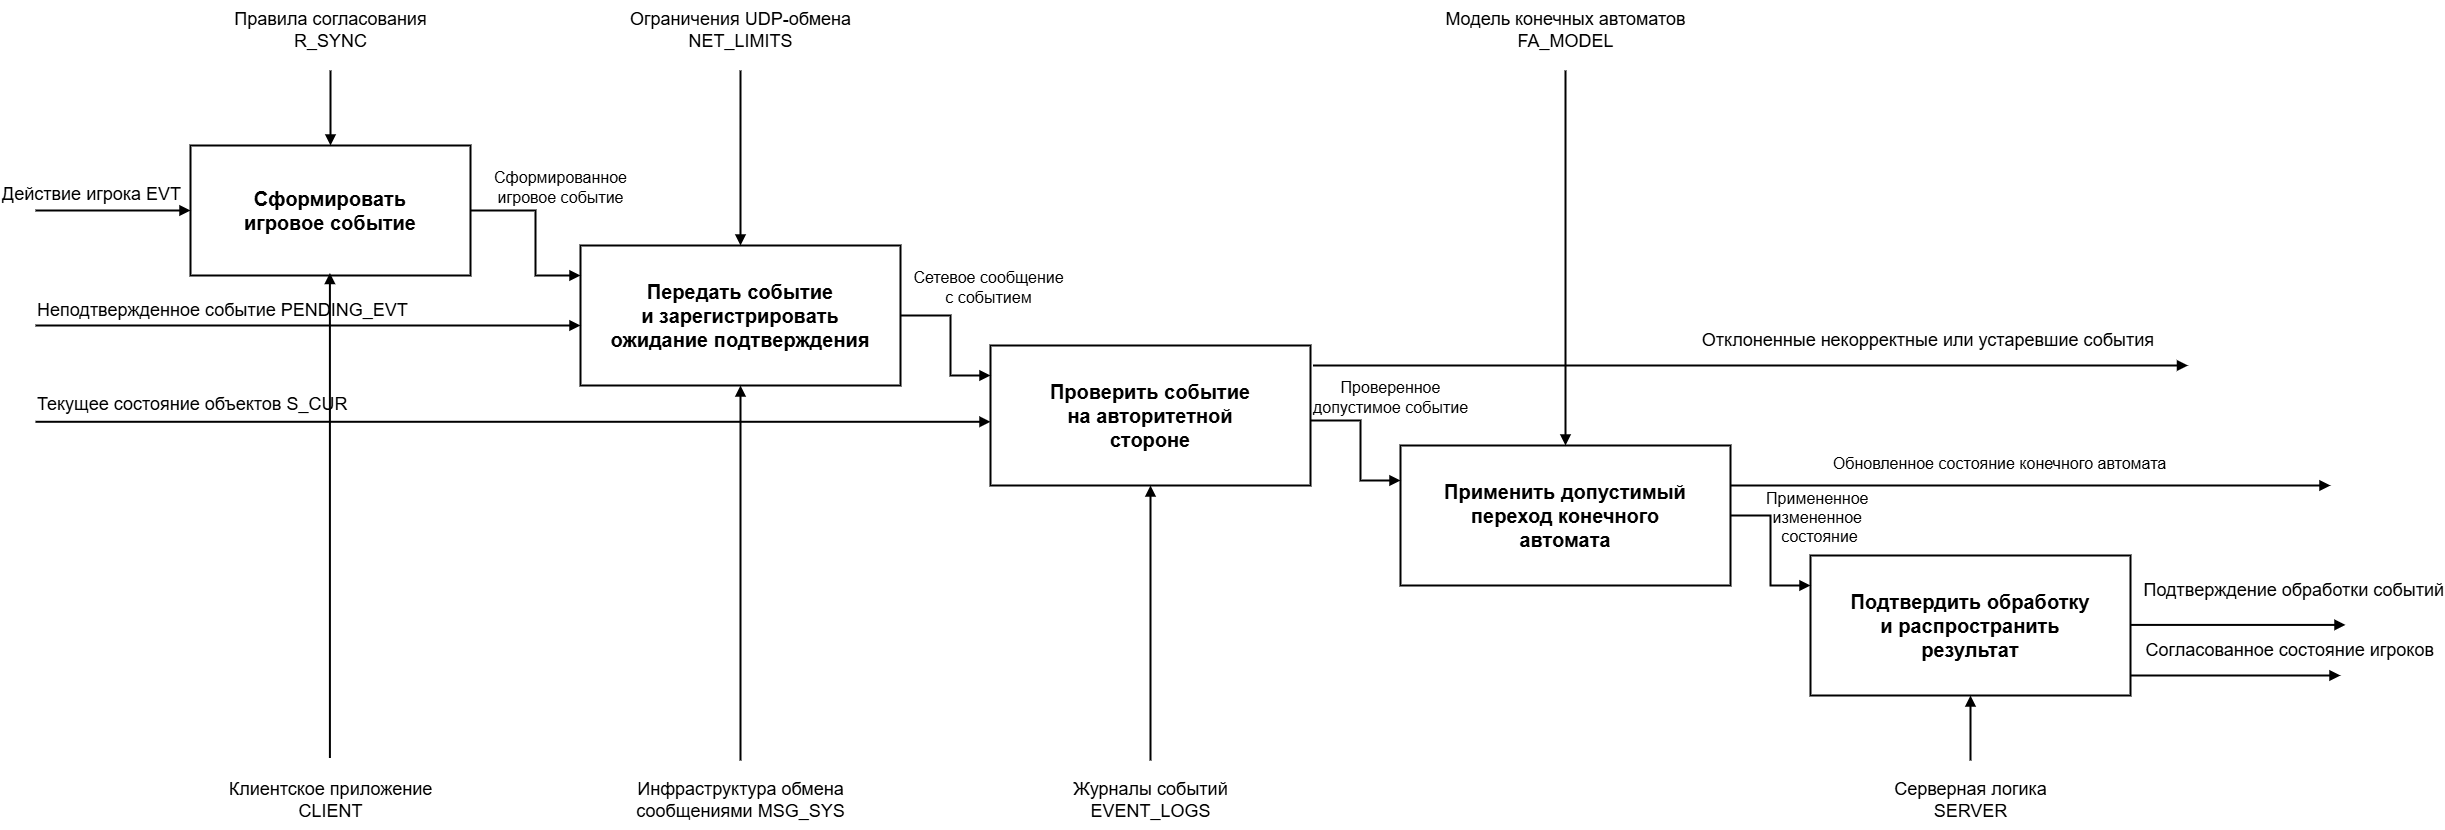
\includegraphics[width=\textwidth]{inc/img/idef1.png}
	\caption{IDEF0-диаграмма метода обеспечения согласованности состояний}
	\label{img:design-idef0}
\end{figure}

\section{Формальная модель синхронизации}

Состояние системы двух игроков в момент времени $t$ зададим как:
\[
	S(t) = \left(S_1(t), S_2(t), O(t), N(t)\right),
\]
где:
\begin{itemize}
	\item $S_1(t)$ --- локальное состояние первого игрока;
	\item $S_2(t)$ --- локальное состояние второго игрока;
	\item $O(t)$ --- множество состояний синхронизируемых игровых объектов;
	\item $N(t)$ --- состояние сетевого протокола синхронизации.
\end{itemize}

Множество синхронизируемых игровых объектов зададим как:
\[
	O = \{o_1, o_2, \ldots, o_n\}.
\]
Каждый объект $o_j$ имеет идентификатор $id(o_j)$ и конечный автомат:
\[
	A_j = \left(Q_j, E_j, \delta_j, q_j^0\right),
\]
где:
\begin{itemize}
	\item $Q_j$ --- множество состояний объекта;
	\item $E_j$ --- множество допустимых событий объекта;
	\item $\delta_j$ --- функция переходов;
	\item $q_j^0$ --- начальное состояние.
\end{itemize}

Игровое событие зададим кортежем:
\[
	e_k = \left(eventId_k, sequence_k, playerId_k, sourceObject_k, targetObject_k, type_k\right),
\]
где:
\begin{itemize}
	\item $eventId_k$ --- уникальный идентификатор события;
	\item $sequence_k$ --- номер события в потоке игрока-отправителя;
	\item $playerId_k$ --- идентификатор игрока-отправителя;
	\item $sourceObject_k$ --- идентификатор объекта-источника;
	\item $targetObject_k$ --- идентификатор целевого объекта;
	\item $type_k$ --- тип события.
\end{itemize}

Сетевое сообщение, передаваемое по UDP, зададим кортежем:
\[
	m_k = \left(messageType_k, event_k, ackId_k, senderId_k, targetId_k\right),
\]
где:
\begin{itemize}
	\item $messageType_k$ --- тип сетевого сообщения;
	\item $event_k$ --- игровое событие;
	\item $ackId_k$ --- идентификатор подтверждаемого события;
	\item $senderId_k$ --- идентификатор отправителя сообщения;
	\item $targetId_k$ --- идентификатор получателя подтверждения.
\end{itemize}

В методе используются три типа сетевых сообщений:
\begin{itemize}
	\item \texttt{ClientHello} --- служебное сообщение регистрации клиента;
	\item \texttt{PuzzleEvent} --- сообщение, содержащее игровое событие;
	\item \texttt{Acknowledgement} --- подтверждение обработки события.
\end{itemize}

Состояние протокола синхронизации на стороне клиента можно представить кортежем:
\[
	N_c = \left(id_c, seq_c^{out}, L_c, A_c\right),
\]
где:
\begin{itemize}
	\item $id_c$ --- идентификатор клиента;
	\item $seq_c^{out}$ --- номер следующего исходящего события;
	\item $L_c$ --- журнал отправленных, но не подтвержденных событий;
	\item $A_c$ --- множество уже примененных событий.
\end{itemize}

Состояние протокола синхронизации на стороне сервера можно представить кортежем:
\[
	N_s = \left(R_s, A_s, H_s\right),
\]
где:
\begin{itemize}
	\item $R_s$ --- множество зарегистрированных конечных автоматов игровых объектов;
	\item $A_s$ --- множество уже примененных событий;
	\item $H_s$ --- отображение идентификатора игрока в номер следующего ожидаемого события.
\end{itemize}

Применение события к игровому объекту определяется функцией:
\[
	Apply(e_k, o_j) =
	\begin{cases}
		true, & \text{если } type_k \in E_j \text{ и переход } \delta_j \text{ допустим};\\
		false, & \text{если событие не может быть применено к объекту}.
	\end{cases}
\]

В таком представлении сетевой уровень передает события, менеджер синхронизации проверяет идентификаторы и порядок сообщений, а допустимость перехода определяется целевым объектом, реализующим конечный автомат.

\section{Состояния протокола синхронизации}

Для описания работы метода выделим следующие состояния протокола синхронизации:
\begin{itemize}
	\item $q_0$ --- регистрация клиента;
	\item $q_1$ --- ожидание локального или сетевого события;
	\item $q_2$ --- формирование исходящего события;
	\item $q_3$ --- ожидание подтверждения;
	\item $q_4$ --- обработка события на сервере;
	\item $q_5$ --- рассылка подтвержденного события;
	\item $q_6$ --- применение подтвержденного события на клиенте;
	\item $q_7$ --- повторная отправка неподтвержденного события;
	\item $q_8$ --- отклонение события.
\end{itemize}

Состояние $q_0$ используется при запуске клиента. Клиент отправляет серверу сообщение \texttt{ClientHello}, содержащее идентификатор игрока. Сервер сохраняет сетевой адрес клиента для последующей рассылки сообщений.

Состояние $q_1$ соответствует обычному режиму работы, в котором клиент ожидает локального действия игрока или входящего сетевого сообщения.

Состояние $q_2$ возникает при локальном действии игрока. Действие преобразуется в событие, которому присваиваются идентификатор и номер последовательности.

Состояние $q_3$ используется после отправки критичного события серверу. Клиент хранит событие в журнале неподтвержденных событий и ожидает подтверждения.

Состояние $q_4$ соответствует обработке события сервером. Сервер проверяет дубликаты, номер последовательности, наличие целевого объекта и допустимость применения события к конечному автомату.

Состояние $q_5$ используется после успешного применения события сервером. Сервер отправляет подтверждение игроку-отправителю и рассылает подтвержденное событие клиентам.

Состояние $q_6$ соответствует обработке подтвержденного события клиентом. Клиент применяет событие к локальному конечному автомату целевого объекта, если событие еще не было обработано.

Состояние $q_7$ возникает при истечении времени ожидания подтверждения. Клиент повторно отправляет событие с теми же значениями идентификатора и номера последовательности.

Состояние $q_8$ используется при получении дубликата, устаревшего события, события с нарушенным порядком или события, которое не может быть применено к целевому конечному автомату.

\begin{figure}[H]
	\centering
	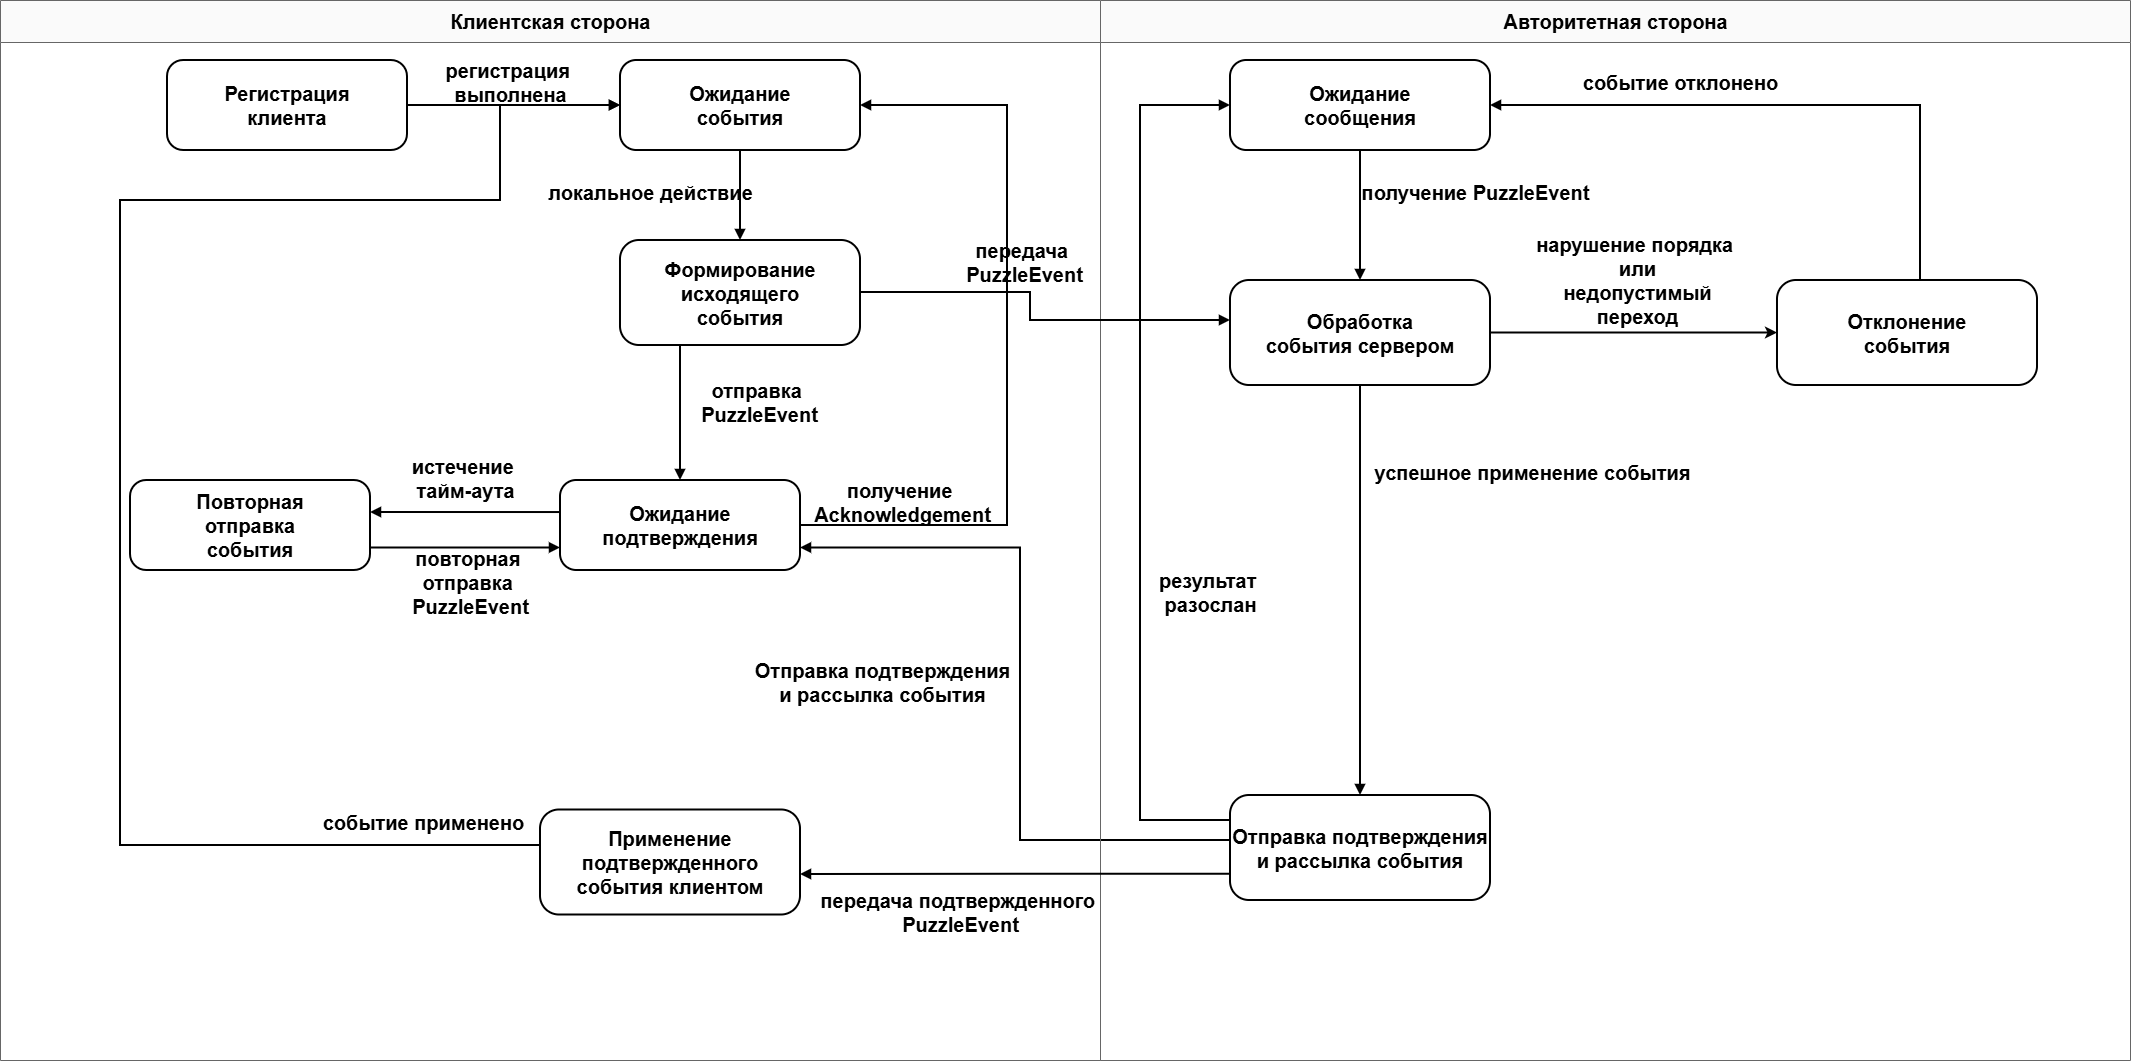
\includegraphics[width=\textwidth]{inc/img/diagram_sync.png}
	\caption{Диаграмма состояний протокола синхронизации}
	\label{img:design-state-machine}
\end{figure}

\section{Модель переходов протокола синхронизации}

Основные переходы протокола синхронизации приведены в таблице~\ref{tab:fsm-transitions}.

{
	\renewcommand{\arraystretch}{1.2}
	\begin{longtable}{|p{3.4cm}|p{4.3cm}|p{3.7cm}|p{3cm}|}
		\caption{Основные переходы протокола синхронизации}
		\label{tab:fsm-transitions}\\
		\hline
		Текущее состояние & Событие & Условие & Следующее состояние \\ \hline
		\endfirsthead
		\hline
		Текущее состояние & Событие & Условие & Следующее состояние \\ \hline
		\endhead
		Регистрация клиента & Отправлен \texttt{ClientHello} & Клиент имеет идентификатор & Ожидание события \\ \hline
		Ожидание события & Локальное действие игрока & Сформирован тип события & Формирование исходящего события \\ \hline
		Формирование исходящего события & Событие отправлено серверу & Событие сохранено в журнале & Ожидание подтверждения \\ \hline
		Ожидание подтверждения & Получен \texttt{Acknowledgement} & Идентификатор события совпадает & Ожидание события \\ \hline
		Ожидание подтверждения & Истек тайм-аут & Событие остается в журнале & Повторная отправка \\ \hline
		Повторная отправка & Событие отправлено повторно & Идентификатор и номер не изменены & Ожидание подтверждения \\ \hline
		Ожидание события & Получен \texttt{PuzzleEvent} сервером & Номер события ожидаемый & Обработка события сервером \\ \hline
		Обработка события сервером & Событие применено к FSM & Переход допустим & Рассылка подтвержденного события \\ \hline
		Обработка события сервером & Событие является дубликатом & Ключ события уже обработан & Отклонение события \\ \hline
		Обработка события сервером & Нарушен порядок & Номер больше ожидаемого & Отклонение события \\ \hline
		\pagebreak
		Рассылка подтвержденного события & Событие отправлено клиентам & Событие принято сервером & Ожидание события \\ \hline
		Ожидание события & Получено подтвержденное событие клиентом & Событие не обработано ранее & Применение события клиентом \\ \hline
		Применение события клиентом & Событие применено к FSM & Переход допустим & Ожидание события \\ \hline
	\end{longtable}
}

Дубликат события не должен приводить к повторному переходу конечного автомата. Если ключ события уже содержится во множестве обработанных событий, состояние объекта не изменяется. На сервере при получении повторного события дополнительно отправляется подтверждение игроку-отправителю, поскольку повтор мог возникнуть из-за потери предыдущего подтверждения.

Если сервер получает событие с номером последовательности меньше ожидаемого, оно рассматривается как устаревшее. Если номер больше ожидаемого, событие не применяется, так как перед ним должно быть обработано одно или несколько предыдущих событий. Такое сообщение не подтверждается, что приводит к повторной отправке со стороны клиента до восстановления корректного порядка доставки.

\section{Структура передаваемых событий}

Передаваемые сообщения делятся на служебные сообщения регистрации, игровые события и подтверждения. Игровые события изменяют состояние конечного автомата целевого игрового объекта. Подтверждения используются для удаления события из журнала неподтвержденных событий клиента.

К игровым событиям относятся:
\begin{itemize}
	\item нажатие интерактивной кнопки;
	\item нажатие или отпускание нажимной плиты;
	\item переключение рычага;
	\item активация моста;
	\item нажатие цветной кнопки;
	\item завершение игровой задачи.
\end{itemize}

Структура игрового события должна включать поля, необходимые для маршрутизации события, контроля порядка и защиты от повторной обработки. В таблице~\ref{tab:event-fields} приведен набор полей события.

\begin{table}[H]
	\caption{Структура игрового события}
	\label{tab:event-fields}
	\centering
	\renewcommand{\arraystretch}{1.2}
	\begin{tabular}{|p{4.5cm}|p{9.5cm}|}
		\hline
		Поле & Назначение \\ \hline
		\texttt{eventId} & Уникальный идентификатор события \\ \hline
		\texttt{sequenceNumber} & Номер события в потоке игрока-отправителя \\ \hline
		\texttt{sourcePlayerId} & Идентификатор игрока-отправителя \\ \hline
		\texttt{sourceObjectId} & Идентификатор объекта, сформировавшего событие \\ \hline
		\texttt{targetObjectId} & Идентификатор объекта, к которому должно быть применено событие \\ \hline
		\texttt{eventType} & Тип игрового события \\ \hline
	\end{tabular}
\end{table}

Структура сетевого сообщения приведена в таблице~\ref{tab:message-fields}.

\begin{table}[H]
	\caption{Структура сетевого сообщения}
	\label{tab:message-fields}
	\centering
	\renewcommand{\arraystretch}{1.2}
	\begin{tabular}{|p{4.5cm}|p{9.5cm}|}
		\hline
		Поле & Назначение \\ \hline
		\texttt{messageType} & Тип сетевого сообщения: \texttt{ClientHello}, \texttt{PuzzleEvent} или \texttt{Acknowledgement} \\ \hline
		\texttt{puzzleEvent} & Игровое событие, передаваемое в сообщении типа \texttt{PuzzleEvent} \\ \hline
		\texttt{ackForEventId} & Идентификатор подтверждаемого события \\ \hline
		\texttt{senderPlayerId} & Идентификатор отправителя сообщения \\ \hline
		\texttt{targetPlayerId} & Идентификатор клиента, которому адресовано подтверждение \\ \hline
	\end{tabular}
\end{table}

Поле \texttt{sequenceNumber} используется для контроля порядка, а поле \texttt{eventId} вместе с \texttt{sourcePlayerId} --- для фильтрации дубликатов. Допустимость перехода не передается в сообщении явно, 
она определяется целевым объектом при вызове метода применения события.


\section{Механизм подтверждения и повторной отправки}

Так как UDP не гарантирует доставку сообщений, надежность для критичных событий обеспечивается на прикладном уровне. После отправки события клиент помещает его в журнал неподтвержденных событий $L_c$. В журнале событие хранится по идентификатору \texttt{eventId}.

Сервер после успешной проверки и применения события отправляет подтверждение. Подтверждение содержит идентификатор принятого события и идентификатор клиента, которому оно адресовано. После получения подтверждения клиент удаляет событие из журнала неподтвержденных событий.

Если подтверждение не получено за время $T_{ack}$, клиент повторно отправляет событие. Повторная отправка не создает новое событие, а использует тот же идентификатор и тот же номер последовательности. Благодаря этому сервер может отличить повторную отправку от нового игрового события.
В разработанном методе повторная отправка продолжается, пока событие находится в журнале неподтвержденных событий.

Последовательность обмена сообщениями в обоих случаях определяется состояниями протокола. После отправки \texttt{PuzzleEvent} клиент переходит в ожидание подтверждения, сервер выполняет авторитетную проверку события, а при отсутствии подтверждения клиент повторно отправляет тот же экземпляр события.

\section{Контроль порядка сообщений}

Для каждого игрока сервер поддерживает номер следующего ожидаемого события. Клиент увеличивает номер последовательности при создании нового логически значимого события. Сервер сравнивает полученный номер с ожидаемым значением.

При получении события возможны следующие случаи:
\begin{itemize}
	\item номер события равен ожидаемому --- событие может быть проверено и применено;
	\item номер события меньше ожидаемого --- событие считается устаревшим или повторным;
	\item номер события больше ожидаемого --- одно или несколько предыдущих событий отсутствуют, поэтому текущее событие не применяется.
\end{itemize}

Для двух игроков достаточно хранить по одному счетчику ожидаемого события на каждого игрока. Это упрощает реализацию по сравнению с системами, где требуется поддерживать множество потоков событий от большого числа участников.

Если событие с большим номером последовательности приходит раньше предыдущих событий, сервер не применяет его и не отправляет подтверждение. Клиент продолжает повторную отправку неподтвержденного события, что позволяет восстановить обработку после доставки недостающего сообщения.

\section{Алгоритм синхронизации состояний}

Схемы алгоритмов обработки исходящего события, серверной обработки события и повторной отправки приведены на рисунках~\ref{img:design-outgoing-event}--\ref{img:design-resend}.

\begin{figure}[H]
	\centering
	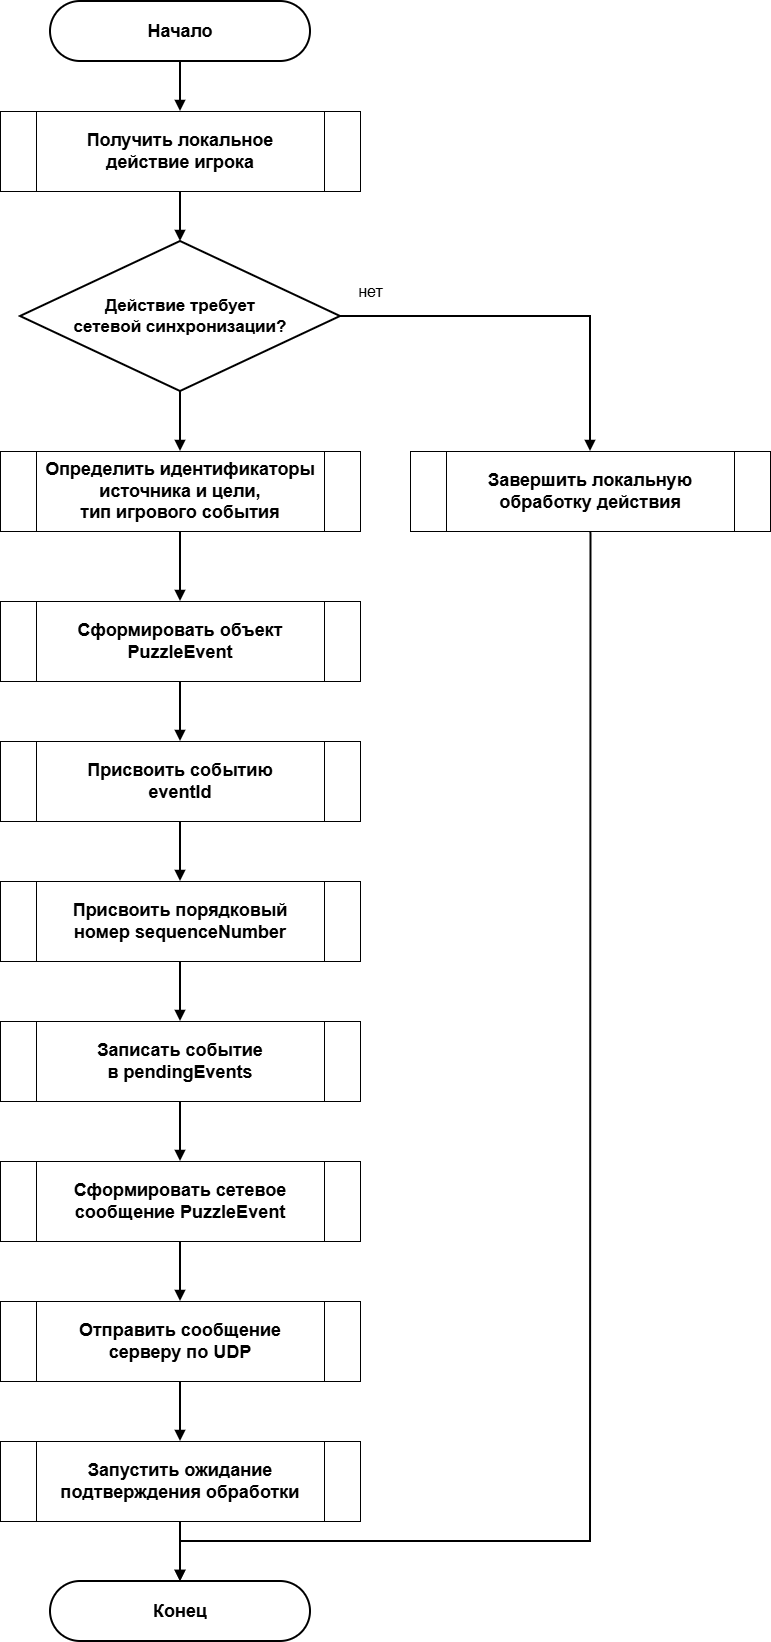
\includegraphics[height=0.82\textheight]{inc/img/outcomming_event.png}
	\caption{Схема алгоритма обработки исходящего события}
	\label{img:design-outgoing-event}
\end{figure}

\begin{figure}[H]
	\centering
	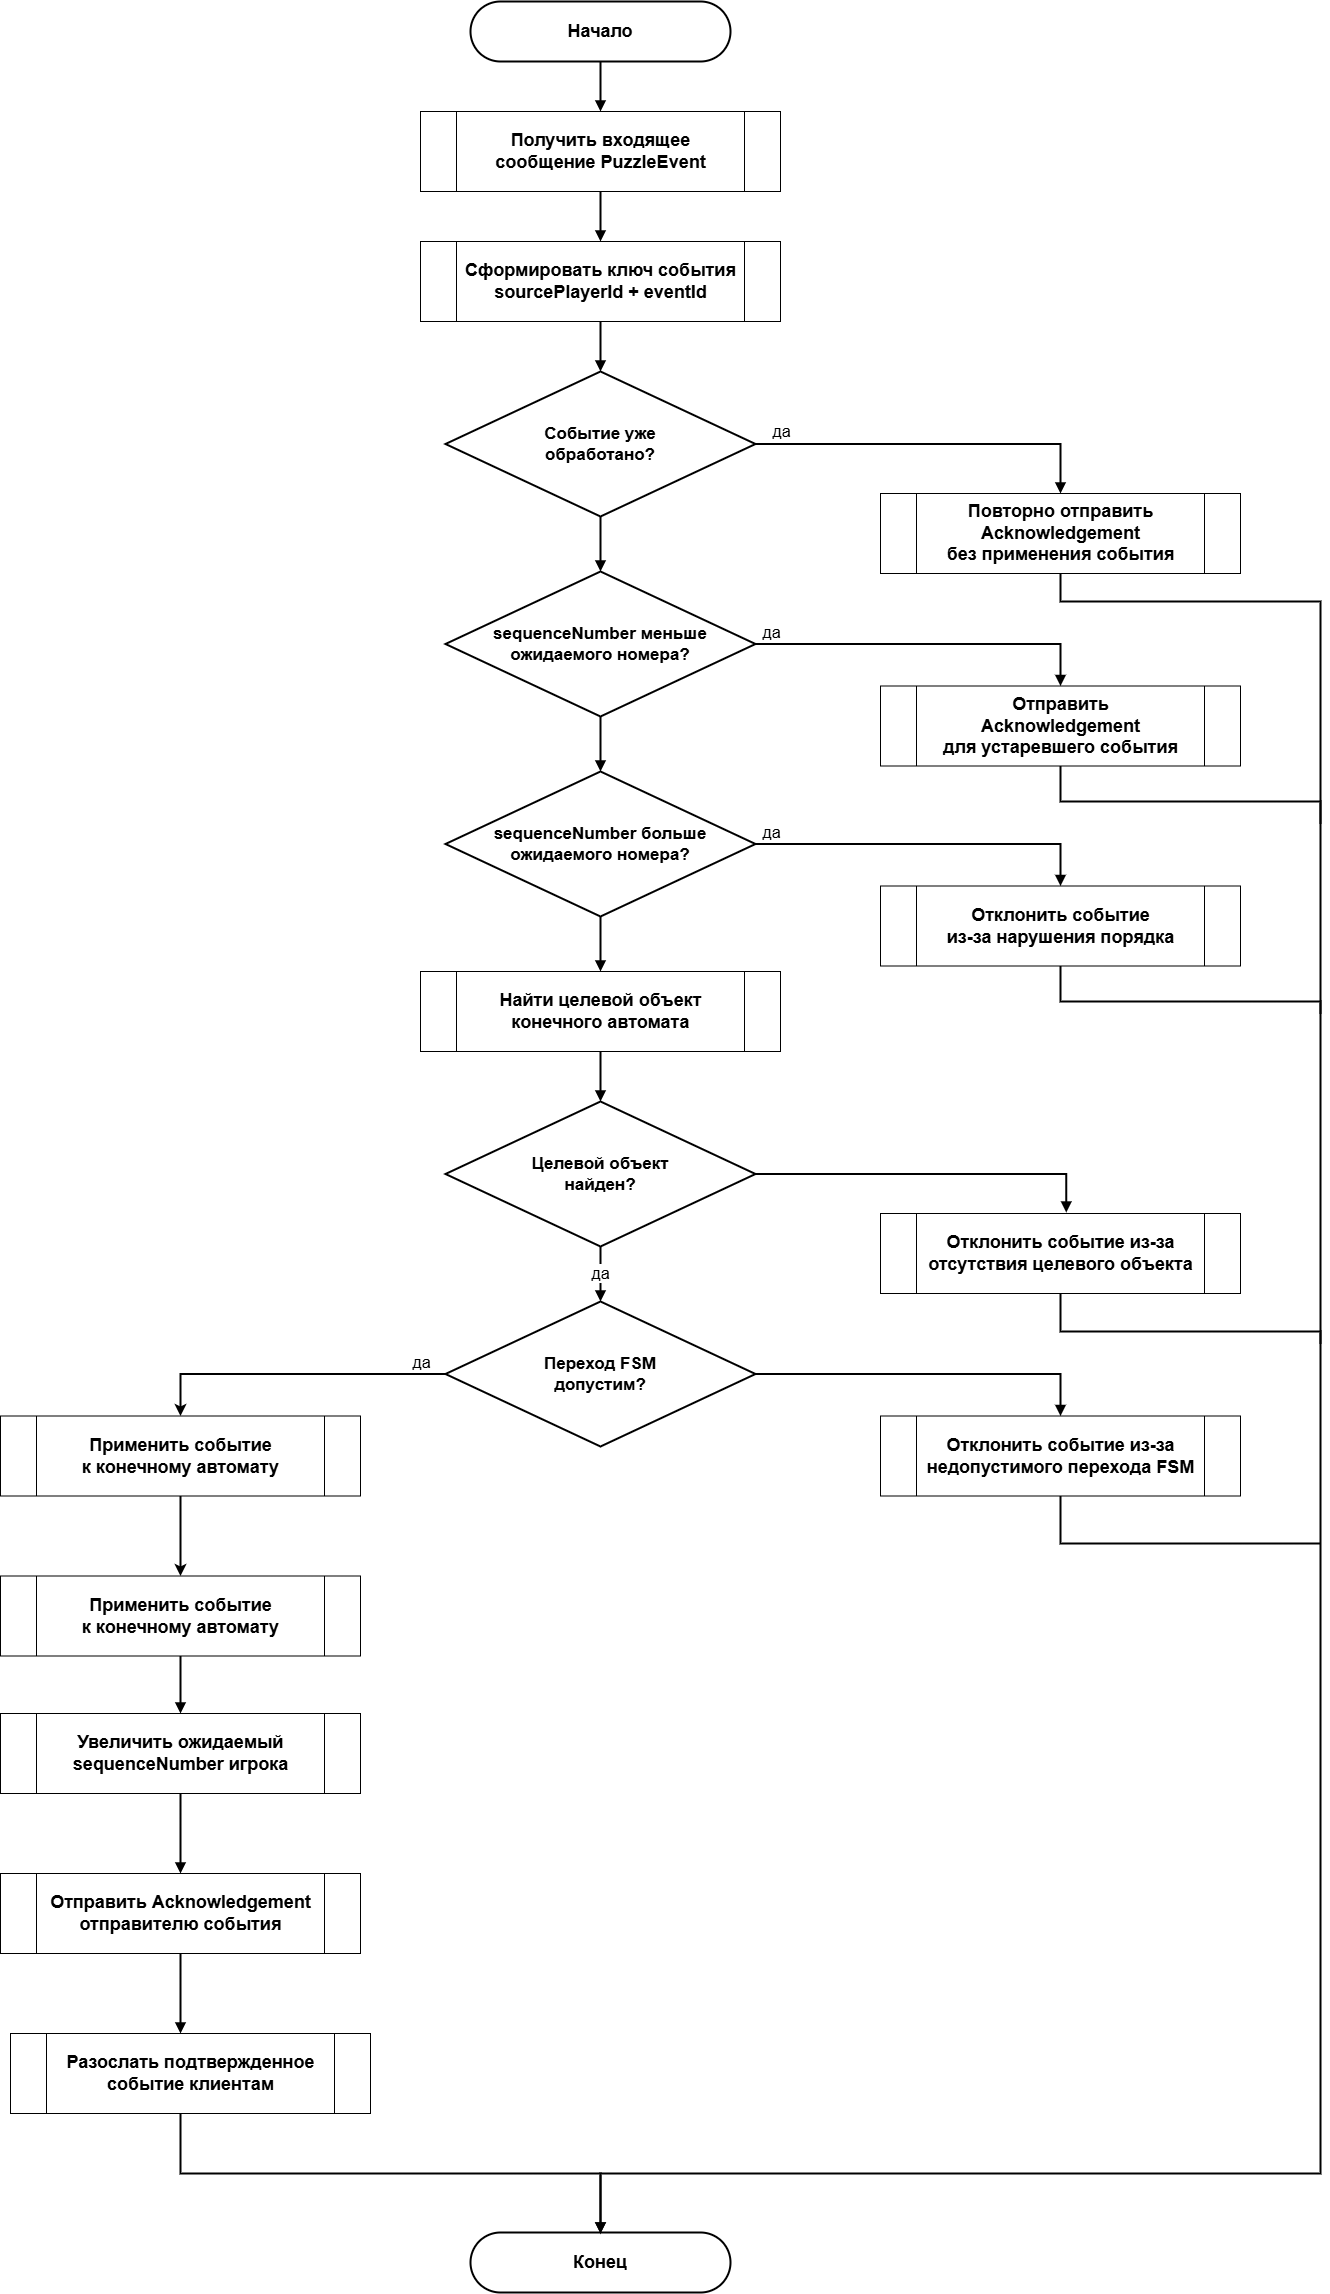
\includegraphics[height=0.82\textheight]{inc/img/server_event.png}
	\caption{Схема алгоритма обработки события сервером}
	\label{img:design-incoming-event}
\end{figure}

\begin{figure}[H]
	\centering
	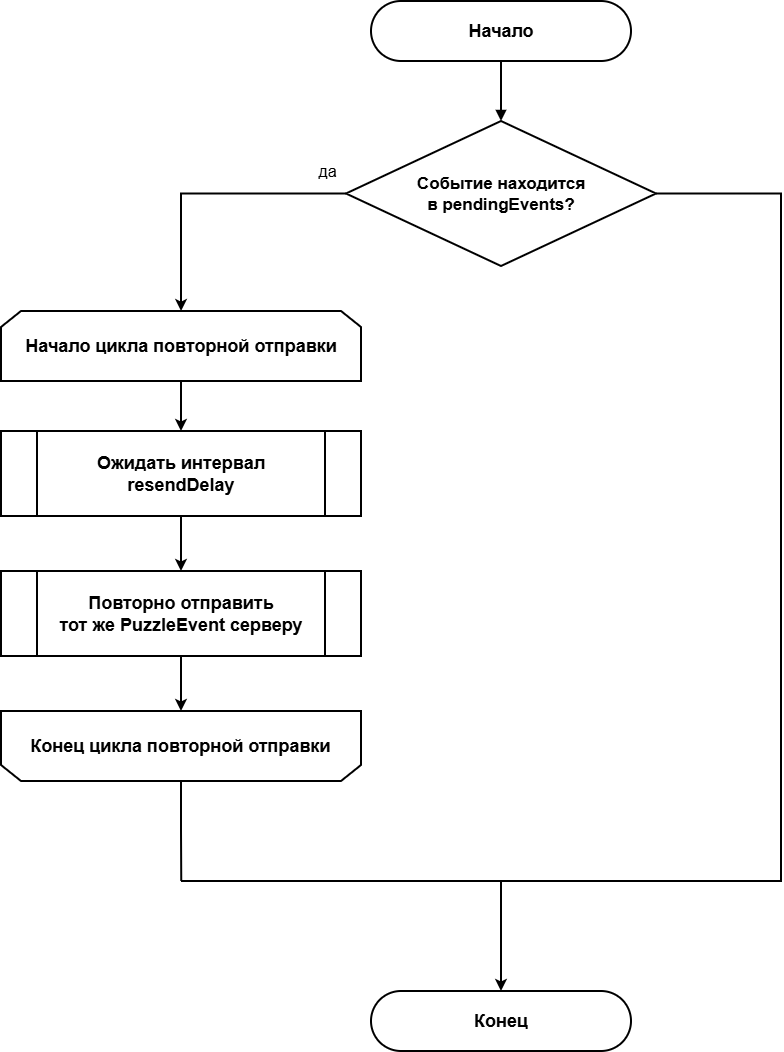
\includegraphics[height=0.72\textheight]{inc/img/recycle_event.png}
	\caption{Схема алгоритма повторной отправки неподтвержденных событий}
	\label{img:design-resend}
\end{figure}

\section{Структура программного обеспечения}

Для реализации предложенного метода разрабатываемое программное обеспечение должно включать следующие компоненты:
\begin{itemize}
	\item модуль сетевого обмена, выполняющий отправку и прием UDP-сообщений;
	\item модуль сериализации и десериализации сетевых сообщений;
	\item журнал неподтвержденных событий клиента;
	\item хранилище обработанных событий для фильтрации дубликатов;
	\item хранилище ожидаемых номеров последовательности на сервере;
	\item менеджер синхронизации событий;
	\item конечные автоматы игровых объектов;
	\item модель игрового состояния двух игроков.
\end{itemize}

Взаимодействие компонентов должно быть организовано так, чтобы сетевой модуль не изменял игровое состояние напрямую. Все входящие сообщения должны передаваться менеджеру синхронизации, который принимает решение о допустимости события и передает его целевому конечному автомату. Это разделяет транспортный уровень и уровень игровой логики, что снижает вероятность некорректного изменения состояния при ошибках сети.


\section*{Вывод}

В данном разделе был разработан метод обеспечения согласованности состояний двух асинхронных игроков с использованием событийной модели и конечных автоматов. 
Были сформулированы требования к методу, определена клиент-серверная функциональная модель синхронизации, задана формальная модель состояния игроков, игровых объектов, событий и сетевых сообщений.

Была предложена структура протокола синхронизации, включающая регистрацию клиента, формирование события, 
ожидание подтверждения, обработку события сервером, рассылку подтвержденного события, применение события клиентом, повторную отправку и отклонение некорректных событий. 
Для модели были описаны основные переходы и условия их выполнения.
